\chapter{Einleitung}
\markboth{1 Einleitung}{}

\section{Problemstellung}
%Unternehmen müssen aufgrund der heutigen dynamischen Veränderungen der Marktgegebenheiten die schnelle Entwicklung ihrer Produkte vorantreiben, sowie deren Platzierung und Bepreisung optimieren.\footnote{Vgl. \cite{gonsch2013using}, S. 94-95\label{dingens1}}
%Das Revenue Management (RM) ist daher für viele Dienstleistungsbereiche unabdinglich geworden. Durch dieses Managementkonzept und den daraus resultierenden Planungsinstrumenten können bei speziellen Anwendungsgebieten die Kapazitätsauslastungen optimiert werden. Damit lassen sich für Unternehmen mit Kapazitätsbe\-schränkungen die Absatzmärkte erfolgreich abschöpfen und die Gesamterlöse maximieren. In dieser Arbeit wird der Ansatz des Verkaufs von opaken Produkten im RM zur besseren Kapazitätsauslastung thematisiert. %\footnote{Klassische Ansätze des RM beschäftigen sich mit der Optimierung der Kapazitätsauslastung bei der Erstellung von Produkten oder Dienstleistungen.}
%Bei opaken Produkten handelt es sich um Produkte, bei denen der Anbieter einige Eigenschaften des Produkts bis zum Abschluss der Transaktion verbirgt.\footref{dingens1} %Anders als bei spezifischen Produkten, bei dem sämtliche Bestandteile der Produkteigenschaften vor dem Kauf bekannt sind.
%Die vorgestellten Produktarten werden i. d. R. in der Dienstleistungsindustrie von multiplen Anbietern angeboten.\footnote{Vgl. \cite{Klein:2008aa}, S. 4} Vereinfacht gesagt bedeutet dies, dass diese Anbieter ihre Dienstleistungen über eine Mehrmarkenstrategie distribuieren und ggf. ihr eigenes Produktportfolio mit anderen Dienstleistungen von Partnerfirmen erweitern. Sie bündeln aus dieser Menge an verfügbaren unterschiedlichen Dienstleistungen ein neues zusammenhängendes Produkt und vertreiben diese Art von Produkten über eine einzelne Marke an potentielle Konsumenten. Aus einem solchen Netzwerk an verfügbaren Produkten kann der Anbieter opake Produkte formen.\footnote{Vgl. \cite{anderson2009effectiveness}, S. 307-309}\textsuperscript{,}\footnote{Siehe Kapitel \ref{DP}}\\Auftragsannahme unter Unsicherheit ist ein kritischer Entscheidungsproblem an der Schnittstelle zwischen Kundenbeziehungsmanagement und Produktionsplanung des auftragsgesteuerten Fertigungssysteme.

Die Entscheidung über die Annahme von Kundenaufträgen unter Unsicherheiten hat weitreichenden Einfluss auf die Produktionsplanung und den Ertrag eines auftragsgesteuerten Fertigungsunternehmens. Ein solches Unternehmen der Auftragsfertigung steht vor dem Entscheidungsproblem, ob der Auftrag zur Produktion des Gutes wirtschaftlich ist. Die Anfragen treffen in beliebiger Reihenfolge ein und haben eine unterschiedliche Wertigkeit. Im weiteren Verlauf dieser Arbeit werden Unternehmen betrachtet, die als auftragsbezogene Dienstleistung das Instandhalten von Güter anbieten. Abhängig des eingehenden Kundenauftrags, indem der Zustand des Gutes beschrieben ist, durch den die notwendigen Prozessschritte zur Instandsetzung des Gutes abgeleitet werden können, generiert das Unternehmen unterschiedliche Erträge. Die Prozessschritte zur Instandsetzung des Gutes geben zusätzlich den notwendigen Ressourcenbedarf für die auszuführende Tätigkeit an, die notwendig sind um das Gut in seinen ursprünglichen bzw. geforderten Zustand zu versetzen. Ressourcen zur Instandsetzung von Gütern können z. B. Material oder Personalstunden sein. Abhängig des möglichen Ertrags und des für den Auftrag notwendigen Ressourcenbedarf muss das produzierende Unternehmen die Entscheidung über Annahme oder Ablehnung des Kundenauftrags treffen. Sofern nur dieser einfache Fall betrachtet wird, bei dem nur der einzelne Kundenauftrag zur Auswahl steht und die Abarbeitung der Aufträge nach der Reihe erfolgt, ist die Entscheidung für das Unternehmen einfach getroffen. Der Kundenauftrag wird angenommen, sofern der Aufwand des Ressourceneinsatzes niedriger als der erziele Ertrag ist.\footnote{In dieser Arbeit wird auf eine differenzierte Betrachtung der Herstellkosten verzichtet.}
Sofern der Unternehmen eine begrenzte Ressourcenkapazität zur Instandsetzung der Güter besitzt, muss zusätzlich der absolute Ressourcenverbrauch des Auftrags für Annahmeentscheidung geprüft werden. Mit Annahme des Auftrags ist ein auftragsbezogener Ertrag erzielt und ein produktbezogener Ressourcenverbrauch eingetreten. Nachdem diese Entscheidung getroffen ist, wird der zeitlich nachfolgende Kundenauftrag betrachtet. Es handelt sich damit um ein klassisches Verfahren des \glqq First-come, first-served (FCFS){\grqq}.

Für die Entscheidung über die Annahme oder Ablehnung eines Kundenauftrags zur Instandhaltung von Gütern bedarf es einer umfassenderen Betrachtung, als nur die kurzsichtige Entscheidung über die Annahme einzelner Aufträge. Angenommen ein Unternehmen der Auftragsfertigung besitzt ein bestimmtes Kontingent an unterschiedlichen Ressourcen über einen bestimmten Zeitraum zur Erfüllung seiner angebotenen Dienstleistung. In diesem betrachteten Zeitraum treffen differenzierte Kundenaufträge mit unterschiedlicher Wertigkeit ein. Zur Maximierung der Erträge über diesen Zeitraum kann es für das Unternehmen sinnvoll sein, Aufträge mit niedrigem Ertrag abzulehnen, sofern im weiteren Verlauf des betrachteten Zeitraums Aufträge mit höherem Ertrag eintreffen. Dies erfolgt in Abhängigkeit der noch vorhanden knappen Ressourcenkapazität, die für die unterschiedlichen Kundenaufträge aufgewendet werden müssen.

Eine weitere Alternative wäre es für das instandhaltende Unternehmen, das zu reparierende Gut mit ein neuwertiges Gut auszutauschen. Es handelt sich damit um eine Entscheidung der Lagerhaltung bei auftragsbezogenen Instandhaltungsprozessen. Die Entscheidung zur Reduzierung des vorhandenen Lagerbestands zur Befriedung des Kundenauftrags im Fokus einer optimalen Kapazitätsauslastung und einer möglichen Ertragsmaximierung macht vor allem Sinn, wenn die zur Produktion notwendigen Ressourcen für spätere Aufträge notwendig sind und mögliche Kapazitäten für die Befriedigung von aktuell geforderten Gutes vorhanden sind. Auch hier kann zwischen dem einfachen Verfahrens des FCFS und eines differenzierten Verfahrens unter Berücksichtigung von zukünftigen Fertigungsaufträgen unterschieden werden. Die kurzfristige Sichtweise untersucht nur den notwendigen Kapazitätsaufwand und den potentiell möglichen Ertrag. Bei der langfristigen Sichtweise unter Berücksichtigung von zukünftigen Anfragen wird der Lagerbestand über einen längeren Zeitraum betrachtet. Sofern in der nahen Zukunft viele Aufträge eintreffen, muss ein solches langfristiges Verfahren eine Entscheidungsunterstützung dem Unternehmen liefern, ob eine Lagerproduktion erfolgen soll. Wie die Bezeichnung der Entscheidung zur Lagerproduktion bereits im Wortlauf deutlich macht, werden die durch den Ressourcenverbrauch geformten Leistungsbündel (Produkte bzw. Dienstleistung) auf Lager produziert. Damit ist es dem Unternehmen möglich zu einem späteren Zeitpunkt die Anfragen mittels des Lagerbestand zu befriedigen.

%%Eine mögliche grafische Darstellungsform dieser Problemstellung erfolgt als sogenannter Entscheidungsbaum. Bei dem Entscheidungsbaum handelt es sich um ein gerichteten azyklischen Graphen. Abhängig der eintreffenden Anfragen, der vorhandenen Kapazitäten, der möglichen Entscheidungen und des betrachteten Zeithorizont hat der Entscheidungsbaum eine unterschiedliche Anzahl an Kanten und Knoten. Ein Knoten bildet jeweils einen neuen Zustand des Systems ab und eine Kante die mögliche Entscheidung in einen neuen Systemzustand zu gelangen.



\section{Zielsetzung}

In dieser Arbeit werden unterschiedliche mathematischen Modell zur Annahmeentscheidung eines Auftrags zur Instandhaltung eines Gutes betrachtet. Dabei werden verschiedene Betrachtungsweisen der Auftragsannahme via Ressourcenkapazität oder Lagerbestand aufgezeigt und untersucht. %Durch Annahme der Entscheidung zur Lagerhaltung des defekten Gutes wird dieses in die Lagerhaltung des Reparaturdienstleisters übernommen und durch ein bereits repariertes Gut ausgetauscht.
Dabei entspricht das reparierte Gut den vom jeweiligen Auftrag geforderten Instandhaltungszustand. Anders formuliert bedeutet dies, dass das produzierende Unternehmen nicht nur die Entscheidungsmöglichkeit über die Instandsetzung des Gutes mittels der Verfügbaren Ressourcenkapazität besitzt, sonder auch die Möglichkeit hat in Abhängigkeit des verfügbaren Lagerbestandes die Kundenaufträge mittels eines neuwertigen Gutes zu befriedigen.

Bei der Problemformulierung der Auftragsannahmeentscheidung bei auftragsbezogenen Instandhaltungsprozessen handelt es sich um ein stochastisch-dynamisches Optimierungsmodell des Netzwerk Revenue Managements. Das Optimierungsmodell trifft die Entscheidung, welche Option zum Lösen des Auftragsannahmeproblems gewählt wird. Das Modell betrachtet dabei den maximal möglichen Erwartungswerts nach Annahme der Option. Als Optionen stehen dem Modell die Auftragsannahme zur Instandsetzung des Gutes, die Auftragsablehnung mit ggf. einer Lagerproduktion von neuwertigen Gütern und die Lagerentnahme eines solchen neuwertigen Gutes zur Verfügung. Diese Entscheidung erfolgt in Abhängigkeit der Veränderung der verfügbaren Ressourcenkapazitäten nach einer möglichen Instandsetzung des Gutes, des aktuell-vorhandenen Lagerbestandes der bereits reparierten Güter und der noch potentiell eintreffenden Anfragen des Netzwerks.

Das Revenue Managements (RM) hat seinen Ursprung in der betrieblichen Problemstellung der Annahme von Aufträgen von freien Sitzplätzen in Passagierflugzeugen.\footnote{Vgl. \cite{talluri2004theory}, S. 6-10.} Das Grundmodell wird zur Annahme von Kundenaufträgen bzw. -anfragen von Dienstleistungsunternehmen mit beschränkten Ressourcenkapazitäten verwendet.\footnote{Vgl. \cite{Petrick:2009aa}, S. 182-187.} %kommt aus der wissenschaftlichen Betrachtung des Revenue Management .
Beim RM wird das Auftragsannehmeproblem der zeitlich nacheinander eintreffenden Produktanfragen als \textit{dynamisch-stochastisches Optimierungsmodell} formulieren und gelöst.
Die Aufgabe des Optimierungsmodells ist laut \cite{talluri2004theory} die Entscheidungsfindung zu unterstützen, damit der Gesamtertrag des Dienstleisters maximiert wird. Der Gesamtertrag wird bewertet in Geldeinheiten (GE). Mit dem Modell lässt sich eine optimale Politik der Auftragsannahme für das betrachtete Netzwerk ableiten.

%Bei den betrachteten Ressourcen handelt es sich um zeitgebundene Ressourcen mit einer jeweiligen vordefinierten Ressourcenkapazität über den gesamten Zeithorizont. 

Die Zielsetzung der Arbeit ist demnach das Grundmodell des Revenue Managements zur Annahme von Kundenaufträgen mit einem Verfahren der Auftragsbefriedigung mittels einer Lagerhaltung von Leistungsbündeln (bzw. Ressourcen) zu erweitern. Zusätzlich zur konzeptionellen Darstellung des hier betrachteten Auftragsannehmeproblems wird für die Modellerweiterung ein Pseudo-Algorithmus entwickelt, welches vorformulierte Beispielszenarien exakt löst. Damit lässt sich eine numerisch Untersuchung durchführen, welche Möglichkeiten sich durch die Betrachtung einer Lagerhaltung in der Auftragsannahme von auftragsbezogenen Instandhaltungsprozessen für Unternehmen ergeben.

\section{Aufbau der Arbeit}

\begin{figure}[h!]
  \begin{center}
    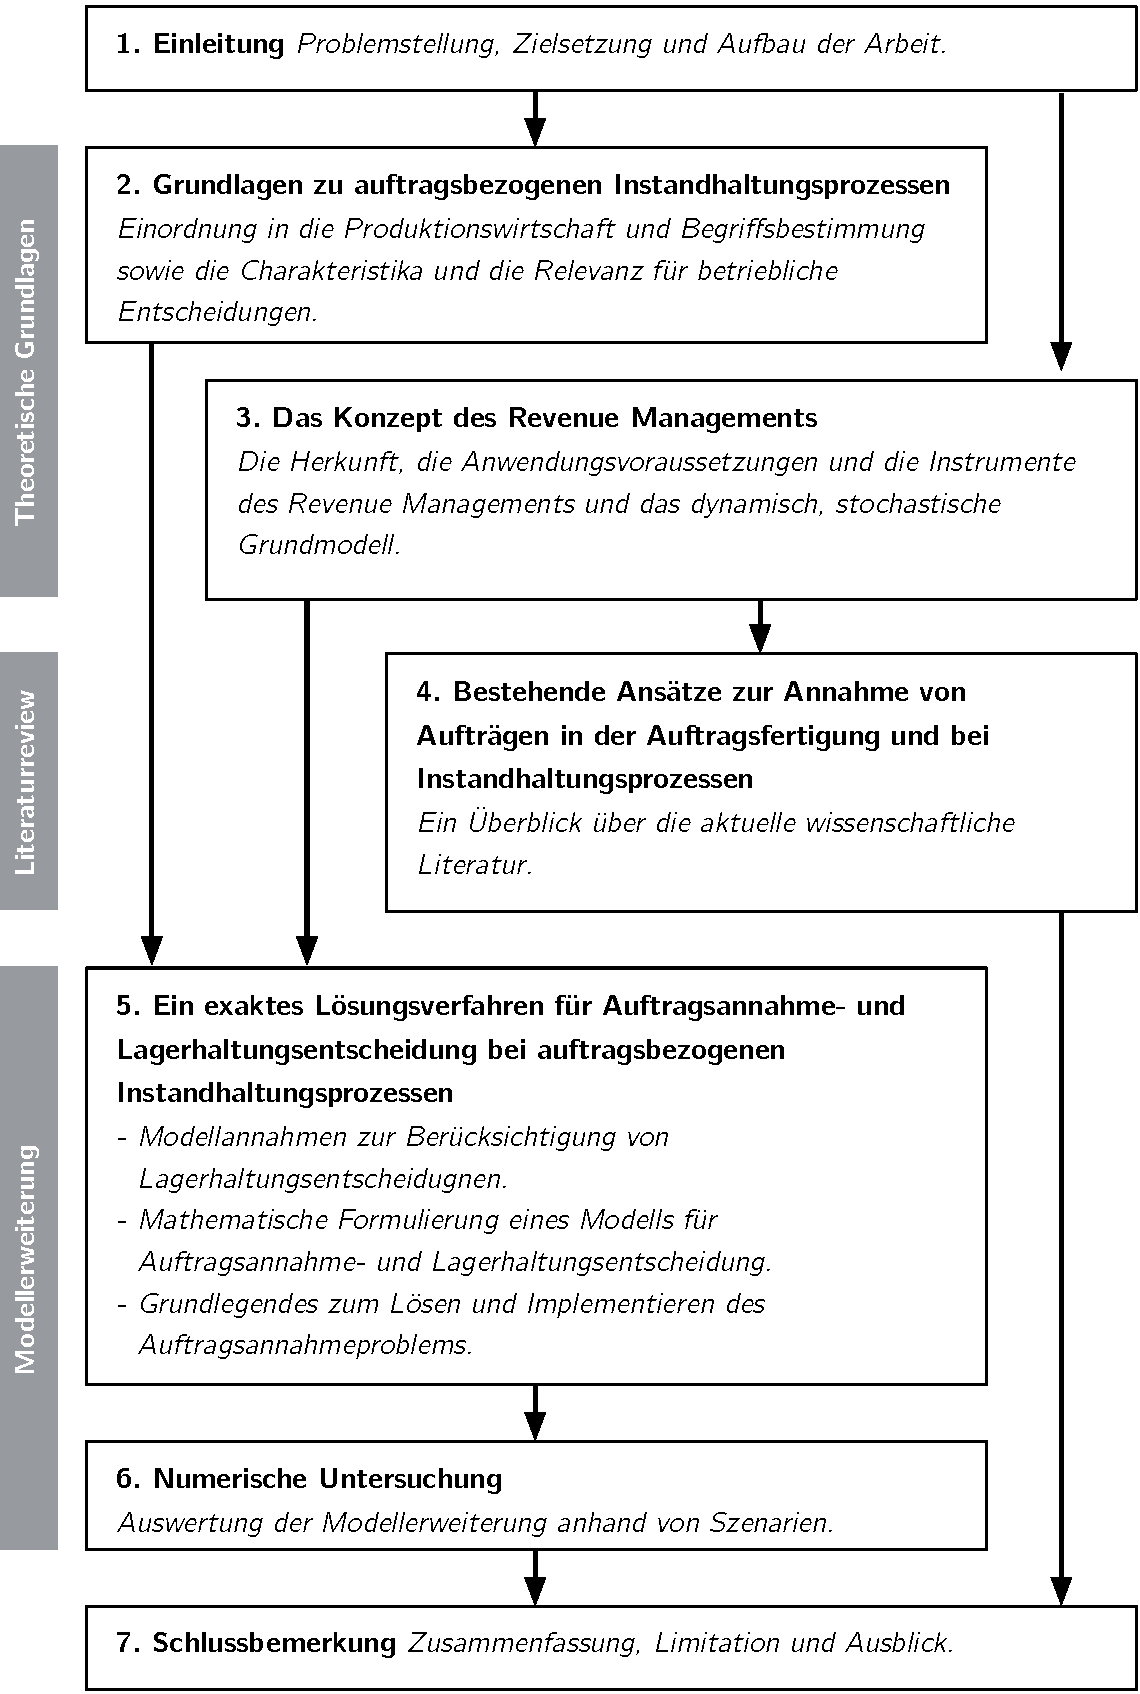
\includegraphics[width=140mm]{Bilder/Gliederung.pdf}
    \caption{Grafische Darstellung der Gliederung der Arbeit}  \label{Gliederung}
  \end{center}
\end{figure}


Der Aufbau der Arbeit ist in der Grafik \ref{Gliederung} dargestellt. In Kapitel 2 wird vorerst der Begriff der auftragsbezogenen Instandhaltungsprozessen definiert und deren theoretische Grundlagen beschrieben. In diesem Kapitel wird der Begriff in die Produktionswirtschaft eingeordnet, sowie die Beschreibung der Charakteristika und der Relevanz für betriebliche Entscheidungen der auftragsbezogenen Instandhaltungsprozessen aufgeführt. Weiter werden im Kapitel 3 die theoretischen Grundlagen der Arbeit vervollständigt, indem das Konzept des Revenue Management bei der Annahme von Aufträgen vorgestellt wird. In diesem Kapitel wird auf die Herkunft des Konzepts eingegangen. Für das Konzept bestehen zusätzlich Anwendungsvoraussetzungen und Instrumente, die in dem Kapitel beschrieben sind. Des Weiteren wird für das Grundmodell des Revenue Managements die mathematische Modellformulierung dargestellt.

Im Anschluss wird in Kapitel 4 ein Literaturüberblick über bestehende Ansätze zur Annahme von Auftragsproduktion und Instandhaltungsprozessen aufgeführt. Es werden hier vier Ansätze näher betrachtet, die den Fokus auf eine heuristische Lösung des Auftragsannahmeproblems legen.

Das Kapitel 5 zeigt die quantitative Untersuchung der Erweiterung des Grundmodells mit der Entscheidung über eine Lagerhaltung auf. Zum einen wird die  mathematische Modellformulierung und zum anderen wird ein Pseudo-Algorithmus zum exakten Lösen der Problemstellung beschrieben. Weiter werden die Grundlagen zur Implementierung des Pseudo-Alorithmus genannt. Im letzten Teil des Kapitels wird auf die numerische Untersuchung eingegangen. Im letzten Kapitel sind die Schlussbemerkungen dieser Arbeit dargestellt. %Es handelt dabei um eine Zusammenfassung der Ergebnisse der vorliegenden Arbeit und um einen Ausblick für nachfolgende Forschung.